\documentclass[12pt,letterpaper]{exam}
\usepackage[lmargin=1in,rmargin=1in,tmargin=1in,bmargin=1in]{geometry}
\usepackage{../style/exams}

% -------------------
% Course & Exam Information
% -------------------
\newcommand{\course}{MAT 108: Exam 2}
\renewcommand{\term}{Fall -- 2022}
\newcommand{\examdate}{11/10/2022}
\newcommand{\timelimit}{85 Minutes}

\setbool{hideans}{true} % Student: True; Instructor: False

% -------------------
% Content
% -------------------
\begin{document}

\examtitle
\instructions{Write your name on the appropriate line on the exam cover sheet. This exam contains \numpages\ pages (including this cover page) and \numquestions\ questions. Check that you have every page of the exam. Answer the questions in the spaces provided on the question sheets. Be sure to answer every part of each question and show all your work. If you run out of room for an answer, continue on the back of the page --- being sure to indicate the problem number.} 
\scores
\bottomline
\newpage

% ---------
% Questions
% ---------
\begin{questions}

% Question 1
\newpage
\question[15] Researchers studying changing viewpoints for youths in education took a survey of 1,001 students in middle school. The researchers asked the students what they believed was the most useful thing in school: having high grades, being popular, or athletic ability. The results, broken down by type of school, are found below. \par
	\begin{table}[!ht]
	\centering
	\begin{tabular}{| l || c | c | c || c |} \hline 
	& Public & Private & Charter & Total \\ \hline \hline
	Grades & 87 & 115 & 82 & 284 \\ \hline
	Popularity & 165 & 91 & 177 & 433 \\ \hline
	Athleticism & 102 & 88 & 94 & 284 \\ \hline \hline
	Total & 354 & 294 & 353 & 1001 \\ \hline
	\end{tabular}
	\end{table} \par
Assuming that this survey is representative of public, private, and charter schools as a whole, determine\dots

\begin{enumerate}[(a)]
\item \dots the percentage of students that attend private schools. 
\item \dots the percentage of students that believe grades are the most useful thing. 
\item \dots the percentage of students that are in charter schools and believe popularity is the most useful thing. 
\item \dots the percentage of students in public schools that believe athleticism is the most useful thing. 
\item \dots the percentage of students in public school, private school, or believe that athleticism is the most important thing. 
\end{enumerate}



% Question 2
\newpage
\question[10] Several medical researchers believe that `genetic drift' is causing the average cholesterol levels in adults to increase. Hence, previously used thresholds of `high cholesterol' may be too low. The researchers measured the cholesterol levels of 265~individuals and found a sample average of 194.1~mg/dL. If cholesterol levels in adults have a standard deviation of 3.8~mg/dL, construct a 92\% confidence interval for the average cholesterol level in adults.



% Question 3
\newpage
\question[10] Mike is playing a D\&D game with a ten-sided die. He comes across a demogorgon---\#FearTheDemogorgon. Unfortunately, the demogorgon has cloned itself, creating 12~copies. Mike needs to roll a 10 to defeat any single demogorgon. 
	\begin{enumerate}[(a)]
	\item Find the probability that Mike defeats exactly two demogorgons.
	\item Find the probability that Mike defeats four or more demogorgons.
	\item Find the probability that Mike defeats all the demogorgons.
	\item Find the probability that Mike defeats at least one of the demogorgons. 
	\end{enumerate}



% Question 4
\newpage
\question[15] Students in a class on quantitative methods in business and social science are studying for an exam. If a student studies, there is an 80\% chance that they will pass the exam. If a student does not study, there is a 75\% chance that they will fail the exam. After a brief survey, the instructors estimates that only 60\% of the students will study for the exam. 
	\begin{enumerate}[(a)]
	\item Find the percentage of the students that will study for the exam and pass.
	\item Find the percentage of students that will fail the exam. 
	\item Find the percentage of students that will pass the exam. 
	\item Find the percentage of students that either did not study or will fail the exam.
	\item What percentage of students that did not study will pass the exam anyway?
	\end{enumerate}



% Question 5
\newpage
\question[10] Students in a class on quantitative methods in business and social science have just taken an exam. The exam scores were normally distributed with a mean of 45 and standard deviation 11.3. 
	\begin{enumerate}[(a)]
	\item Find the percentage of students that scored at least 65 on the exam. 
	\item Find the minimal score one would need to be in the top 10\% of exam scores. 
	\end{enumerate}



% Question 6
\newpage
\question[10] Local government officials are trying to determine how to allocate public health funds from a recent grant. It is known that approximately 26\% of adults in the US have some type of disability. One of the villages in the county has a population of 2,500 adults.
	\begin{enumerate}[(a)]
	\item What is the probability that less than 620 of these adults will have a disability?
	\item What is the probability that less than 720 of these adults will have a disability?
	\item What is the probability that between 620 and 720 of these adults will have a disability?
	\end{enumerate}



% Question 7
\newpage
\question[10] A researcher is collecting data on sleep and academic performance. They collect data on student's GPA, $g$, and plot it against the average number of hours of sleep, $h$, students had during a given week. They find a linear regression model of $\widehat{g}= 0.028h + 3.5$. A scatterplot of their data with the model is found below.
	\begin{figure}[!ht]
	\centering
	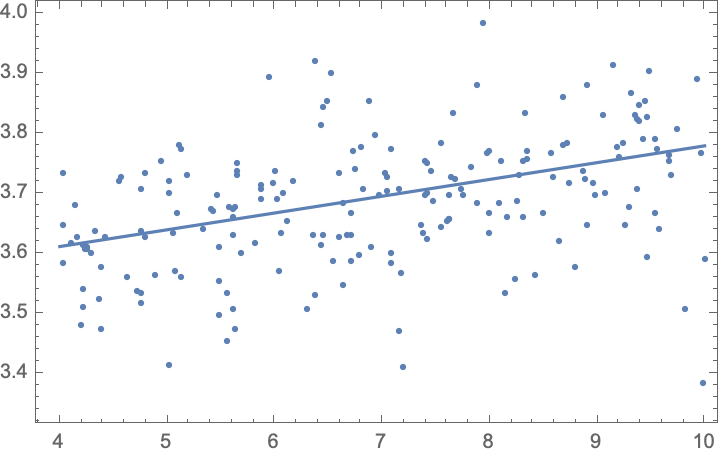
\includegraphics[width=0.48\textwidth]{regplot.png}
	\end{figure}

\begin{enumerate}[(a)]
\item Find the model's prediction of a student's GPA if they slept 8~hours a night.
\item If a student that slept 8~hours a night had a GPA of 3.528, find the residual for this model's prediction of this datapoint. 
\item If the researchers had an $R^2$ value of 0.407263, does this imply a `good' model, i.e. a strong correlation? Explain.
\item Is (c) supported by the scatterplot above? Explain.
\end{enumerate}



% Question 8
\newpage
\question[10] A company claims that their warehouse workers are paid more than the national average of \$23.75 per hour. A local journalist doubts the company's claim and surveys 15 of the workers at the warehouse about their hourly wage. The journalist assume that wages at the warehouse have the same standard deviation of \$1.27 as wages nationally for this type of job.
	\begin{enumerate}[(a)]
	\item Find the probability that the average salary of these workers is less than \$23 per hour.
	\item What assumption(s) about the workers' salary do your calculations in (a) require, if any. 
	\end{enumerate}



% Question 9
\newpage
\question[10] Read the following two scenarios:
	\begin{enumerate}
	\item[I.] A politician is making claims about immigrants into their country. They cite data showing that $68.3\%$ of these immigrants do not have higher education. Because studies have shown that $4.12\%$ of those without higher education will commit violent crimes, they claim that $68.3 \cdot 4.12 \approx 2.81\%$ of these immigrants will commit a violent crime. They also claim that because there were $10,000$ new immigrants last month, there are now $10,\!000 \cdot 0.0281 \approx 281$ new violent criminals in the area.
	\item[II.] Efficiency managers have been hired at a local law firm to improve `work flow' at their company. The efficiency managers gather data and find that $40\%$ of workers handle some type of paperwork while $33\%$ of workers handle some type of data entry. They conclude that at least $40\% + 33\%= 73\%$ of workers at the company either handle some type of paperwork or some type of data entry. 
	\end{enumerate}
Now respond to the following two questions:

\begin{enumerate}[(a)]
\item Is the mathematical claim the politician made in (I) correctly reasoned? Explain.
\item Is the mathematical claim the efficiency managers made in (II) correctly reasoned? Explain.
\end{enumerate}




















\end{questions}
\end{document}